%------------------------------------------------
% main.tex - Test file for LatexTree package
%------------------------------------------------
\documentclass[oneside, 11pt]{book}

% document info
\title{Test Book for the LatexTree Package}
\author{D Evans}
\date{June 2017}

% standard packages
\usepackage{amsmath,amsfonts,amsthm}
\usepackage{geometry}
\usepackage{graphicx}
\usepackage{subfigure}
\usepackage{caption}
\usepackage{fancyhdr}

% package parameters
\geometry{margin=20mm, a4paper}
\graphicspath{{figures/}}

% theorem definitions
\newtheoremstyle{cumaths}{}{}{\upshape}{}{\bfseries}{~}{\newline}{}
\theoremstyle{cumaths}
\newtheorem{theorem}{Theorem}[chapter]
\newtheorem{definition}[theorem]{Definition}
\newtheorem{lemma}[theorem]{Lemma}
\newtheorem{example}[theorem]{Example}
\newtheorem{exercise}[theorem]{Exercise}
\newtheorem{corollary}[theorem]{Corollary}
\newtheorem{remark}[theorem]{Remark}
\renewcommand{\thetheorem}{\arabic{chapter}.\arabic{theorem}}

% new normalmode commands
\renewcommand{\emph}[1]{\textbf{#1}}

% new mathmode commands
\newcommand{\N}{\mathbb{N}}
\newcommand{\Z}{\mathbb{Z}}
\newcommand{\R}{\mathbb{R}}
\newcommand{\C}{\mathbb{C}}
\newcommand{\prob}{\mathbb{P}}
\newcommand{\expe}{\mathbb{E}}
\newcommand{\var}{\text{Var}}
\newcommand{\cov}{\text{Cov}}
\DeclareMathOperator*{\argmin}{\arg\!\min}
\DeclareMathOperator*{\argmax}{\arg\!\max}

% TeX aliases (these are expanded by latextree prior to parsing).
\def\it{\item}
\def\bit{\begin{itemize}}
\def\eit{\end{itemize}} 
\def\ben{\begin{enumerate}}
\def\een{\end{enumerate}}

% videos
\newcommand{\includevideo}[2][1]{\url{#2}}
\usepackage{newfloat}
\usepackage{caption}
\DeclareFloatingEnvironment[placement={!ht},name=Video]{video}
\captionsetup[video]{labelfont=normalfont}

% tweaks
\setlength{\parindent}{0ex}
\setlength{\parskip}{1ex}
\renewcommand{\arraystretch}{1.3}
\addtolength{\tabcolsep}{2ex}

% hyperref (always load last)
\usepackage{hyperref}
\hypersetup{colorlinks=true, linkcolor=blue}

%----------------------------------------
\begin{document}\label{book:latextreetest}
\maketitle
\tableofcontents
\newpage

\pagestyle{plain}
\chapter*{Preface}
This is a test document for the {\tt LatexTree} package. 

\pagestyle{fancy}
% !TEX root = main.tex

\chapter{Levels and Headings}\label{ch:levels}

Text can be included before the first section (like the preface to the document).

\section{First section}\label{sec:first}
Text in the first section of the chapter.

\subsection{A fancy title: $\alpha + \beta$}\label{subsec:fancy}
Text in the first subsection of the first section.

\section{Second section}\label{sec:second}
Text in the second section.

\section{Headings}
The starred macros \texttt{chapter*}, \texttt{section*} and \texttt{subsection*} yield simple headings. They are not numbered and do not feature in the table of contents. 

\section*{A section-level heading}
Some text.

\subsection*{A subsection-level heading}
Some more text.
\endinput


% !TEX root = main.tex

\chapter{Lists}

An unordered list:
\begin{itemize}
\item Apples
\item Oranges
\item Lemons
\end{itemize}

An ordered list:
\begin{enumerate}
\item Cars
\item Buses
\item Bikes
\end{enumerate}

\endinput


% !TEX root = main.tex

\chapter{Mathematics}

Note: MathJax refuses to display two equations with the same label on the same page. 

%--------------------
\section*{Equations}

An inline equation: $\sum_{n=1}^{\infty} a_n = 1$.

An \texttt{equation} environment:
\begin{equation}
\sum_{n=1}^{\infty} a_n = 1.
\end{equation}

An \texttt{equation*} environment:
\begin{equation*}
\sum_{n=1}^{\infty}\frac{1}{n^2} = \frac{\pi^2}{6}.
\end{equation*}

A \texttt{displaymath} environment:% using \texttt{\textbackslash[} and \texttt{\textbackslash]}:
\[
x = \frac{-b\pm\sqrt{b^2-4ac}}{2a}.
\]

A \texttt{displaymath} environment containing a \texttt{text} macro, which itself contains mathmode:
\[
E=mc^2 \text{ where $c$ is the speed of light}.
\]

%The quadratic formula shown inline: $x = \frac{-b\pm\sqrt{b^2-4ac}}{2a}$. 

%--------------------
\section*{Labelled equations}


An equation with a label:
\begin{equation}\label{eq:euler}
e^{i\pi}+1=0.
\end{equation}

Equation -\eqref{eq:euler}- is due to Euler.

An \texttt{align} environment:
\begin{align}\label{eq:ellipse}
x & = a\sin\theta \\
y & = b\cos\theta
\end{align}

\bigskip
An \texttt{align*} environment:
\begin{align*}
x & = a\sin\theta \\
y & = b\cos\theta
\end{align*}

%\bigskip
%A labelled \texttt{equation} environment:
%\begin{equation}\label{eq:einstein}
%E = mc^2
%\end{equation}
%Equation -\eqref{eq:einstein}- is due to AE. 

\bigskip
An {\tt equation} containing three {\tt pmatrix} environments:
\begin{equation}
\begin{pmatrix}0 & 1 \\ 1 & 0\end{pmatrix}
\qquad
\begin{pmatrix}0 & -i \\ i & 0\end{pmatrix}
\qquad
\begin{pmatrix}1 & 0 \\ 0 & -1\end{pmatrix}
\end{equation}

A displayed equation using double-dollars:
$$
F = ma
$$
{\tt LatexTree} deals with these during pre-processing.
\endinput


% !TEX root = main.tex

\chapter{Theorems}

\begin{theorem}
If $a$ and $b$ are odd numbers, then $ab$ is an odd number.
\begin{proof}
Let $a$ and $b$ be odd numbers. Then by definition there exist integers $c$ and $d$ such that 
\[
a=2c+1 \quad\text{and}\quad b=2d+1.
\]

It is easy to show that $ab = 2(2cd + c + d) + 1$, and because $2cd+c+d$ is an integer we conclude that $ab$ is odd.
\end{proof}
\end{theorem}

\begin{theorem}
$\sqrt{2}$ is irrational.
\begin{proof}
Suppose to the contrary that $\sqrt{2}$ is rational. Let us write $\sqrt{2} = a/b$ where $a$ and $b$ are integers, and assume that the fraction is written in its simplest terms.
Then we have $2b^2 = a^2$ which implies that $a^2$ is even.
\par
By the previous theorem, if $a$ is odd then $a^2$ is also odd, so it must be that $a$ is even. Let us write this as $a=2c$ for some integer $c$. Then
\[
2b^2 = a^2 = (2c)^2 = 4c^2, \text{ so } b^2 = 2c^2.
\]
As above we conclude that $b$ must also be even, i.e.\ $b = 2d$ for some integer $d$.
\par
We assumed however that the fraction $a/b$ was in its simplest form, but we have shown that this is not the case, because
\[
\sqrt{2} = a/b = (2c)/(2d) = c/d.
\]
This is a contradiction, so we conclude that $\sqrt{2}$ is irrational.
\end{proof}
\end{theorem}


\begin{theorem}
There are infinitely many prime numbers.
\begin{proof}
Assume the contrary statement: suppose that there are only finitely many prime numbers. Call them $p_1,p_2\ldots,p_n$.
Then the number $p = p_1p_2\ldots p_n + 1$ is bigger than all of $p_1,p_2,\ldots,p_n$ and so cannot be prime.
\par
If we divide $p$ by any of the $p_j$ we get remainder $1$, so $p$ must be divisible by some non-prime number, say $b$.
By the Fundamental Theorem of Arithmetic, every integer greater than $1$ is either prime or the product of prime numbers.
\par
Consequently there must be a prime number $p_j$ that divides $b$, and which therefore divides $p$.
This is a contradiction, so our original assumption must be false.
Thus we conclude that there are infinitely many prime numbers.
\end{proof}
\end{theorem}
% !TEX root = main.tex

\chapter{Text Processing}

\section{Spacing problems}
Here is a sum $1+1=2$. Watch the comma $\sum x_n^2$, is there a space? Seems to be fixed!

\subsection*{Non-breaking spaces}
Tildes don't appear in mathmode. Here is an fbox containing lots of them:
\par
\fbox{$A~~~~~~~~~~~~~~~~~~~~~~~~~~~~~~~~~~~~~~~~~~~~~~~~~~~~~~~~~~~~~~~~~~~~~~~~~~~~~~~~~~~~~~~~~~~~~~~~~~~~~~B$}
\par

\bigskip
The {\tt LatexTree} parser replaces
\bit
\it all tildes in normal mode by (non-breaking) spaces and
\it all spaces in mathmode by tildes (to foil Blackboard's rewriters).
\eit


\section{Accents and escaped characters}

\subsection*{Accents}
Spaces between consecutive characters are disappear after processing. This is a consequence of not leaving a space between consecutive text elements. (This can be fixed by merging adjacent text elements, perhaps during post-processing.)
\bit
\it These should be spaced: \'{e} \`{e} \^{w} \"{o} \c{c}.
\it We can manually input the spaces: \'{e}\ \`{e}\ \^{w}\ \"{o}\ \c{c}.
\eit
All seems fine for accented characters inside words:
\bit
\it Cram\'{e}r-Rao.
\it Y m\^{o}r coch.
\it He is blas\'{e} about it.
\eit

\subsection*{Escaped characters}
Here are some escaped characters:
\bit
\it ampersand: \& 
\it percent: \%
\it dollar: \$
\eit

We need to be careful with \$ characters!

\section{Font styles}
Here are some font styles: 
\bit
\it \textbf{bold}
\it \textit{italic}
\it \texttt{teletype}
\it \textsc{small caps} 
\it \textsl{oblique}
\it \emph{emphasis}
\eit

\section{TeX shortcuts for lists}
The itemize macros (\texttt{bit,it,eit}):
\bit
\it apples
\it oranges
\eit

The enumerate macros (\texttt{ben,it,een}):
\ben
\it first
\it second
\een

{\tt LatexTree} deals with these during pre-processing.


% !TEX root = main.tex

\chapter{Tables}

\subsection*{Inline}
An inline \texttt{tabular} environment:
\begin{tabular}{|ccc|}\hline
$\alpha$ & $\beta$ & $\gamma$ \\ \hline
$1/2$ & $1/3$ & $1/6$ \\ \hline
\end{tabular}

\subsection*{Centred}
A centred \texttt{tabular} environment:
\begin{center}
\begin{tabular}{|c|c|c|}
\hline
(1,1) & (1,2) & (1,3) \\
\hline
(2,1) & (2,2) & (2,3) \\
\hline
\end{tabular}
\end{center}

\subsection*{Floating}
A floating \texttt{table} environment:
\begin{table}[htb]
\centering
\begin{tabular}{|c|c||c|c|c|} \hline
Set Theory 		& 			& Logic			&		& \\ \hline
Union			& $A\cup B$	& Disjunction 	& OR 	& $\lor$	\\
Intersection		& $A\cap B$	& Conjunction	& AND 	& $\land$\\
Complement		& $A^c$		& Negation		& NOT 	& $\lnot$	\\ \hline
\end{tabular}
\caption{Logic and Set Theory}
\end{table}



% !TEX root = main.tex

\chapter{Images and Video}

\section{Images}

We parse the optional argument to \texttt{includegraphics}. The \texttt{Image} class has an attribute \texttt{width} expressed as a percentage. This is computed from the (optional) \texttt{scale} or \texttt{width} parameters passed to \texttt{includegraphics}.

\begin{itemize}
\item \autoref{fig:acapb} is the original (scale = 0.25).
\item \autoref{fig:acapb-big} is the big one (scale = 0.5).
\item \autoref{fig:acapb-small} is the small one (scale = 0.1).
\item \autoref{fig:setops-subfig} shows a figure layout using \texttt{subfigure}.
\item \autoref{fig:setops-tabular} shows a figure layout using \texttt{tabular}. %The optional parameter to \texttt{includegraphics} is \texttt{scale=0.4}, and the pictures take up 40\% of each cell, which is a pity.
\end{itemize}

\begin{figure}[ht]
\centering
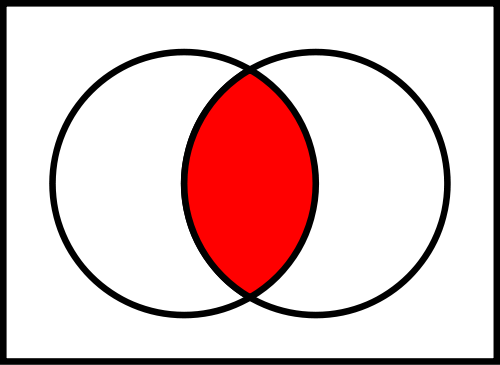
\includegraphics[scale=0.25]{AcapB}
\caption{Set intersection (scale=0.25)\label{fig:acapb}}
\end{figure}

\begin{figure}[ht]
\centering
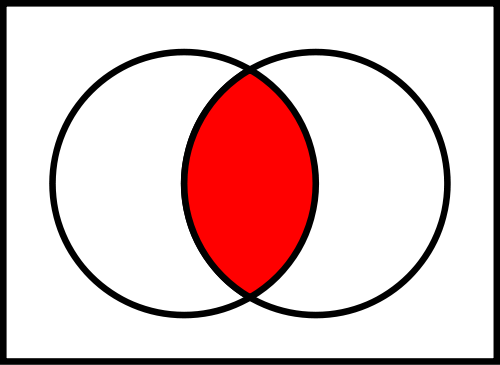
\includegraphics[scale=0.5]{AcapB}
\caption{The big one (scale=0.5)\label{fig:acapb-big}}
\end{figure}

\begin{figure}[ht]
\centering
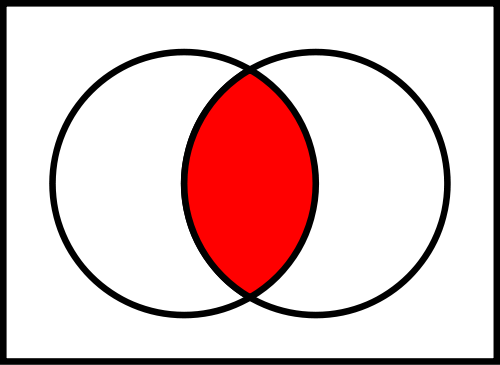
\includegraphics[scale=0.1]{AcapB}
\caption{The small one (scale=0.1)\label{fig:acapb-small}}
\end{figure}

\begin{figure}[htb]
\centering
\subfigure[Union]{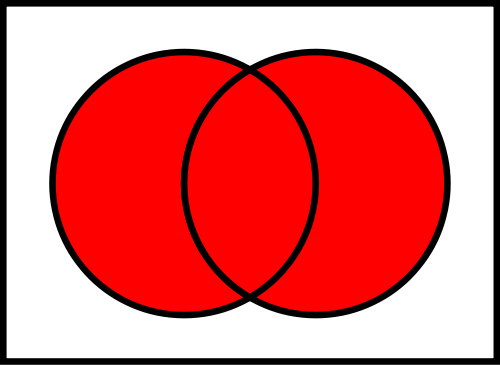
\includegraphics[scale=0.25]{AcupB}\label{fig:union}}
\subfigure[Intersection]{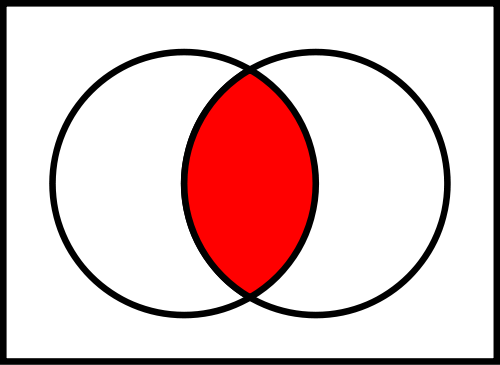
\includegraphics[scale=0.25]{AcapB}\label{fig:intersection}}
\subfigure[Complement]{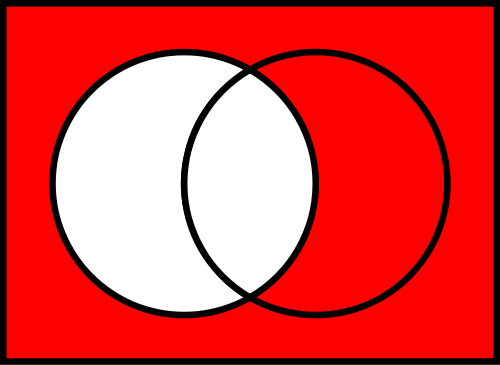
\includegraphics[scale=0.25]{Acomp}\label{fig:complement}}
\caption{Three figures using \texttt{subfigure}.\label{fig:setops-subfig}}
\end{figure}

\begin{figure}[htb]
\centering
\begin{tabular}{ccc}
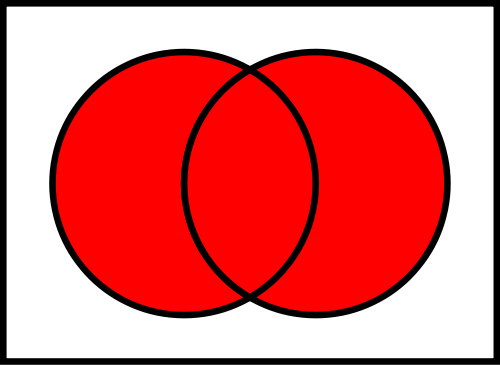
\includegraphics[width=0.25\linewidth]{AcupB} &
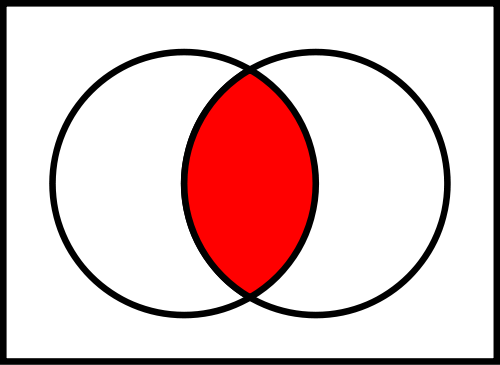
\includegraphics[width=0.25\textwidth]{AcapB} &
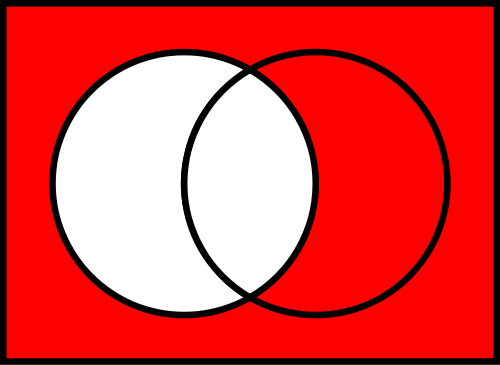
\includegraphics[width=0.25\textwidth]{Acomp} \\
(a) Union & (b) Intersection & (c) Complementation \\
\end{tabular}
\caption{Three figures using \texttt{tabular}.\label{fig:setops-tabular}}
\end{figure}

%--------------------
\section{Videos}
Embedding videos in PDFs is not easy and not recommended. Instead we include hyperlinks links using the \texttt{url} and \texttt{href} macros. 


\subsection{The \texttt{url} macro}
Please watch this video: \url{https://www.youtube.com/watch?v=oCDXhvXye9E}.

\subsection{The \texttt{href} macro}
Please watch this \href{https://www.youtube.com/watch?v=oCDXhvXye9E}{video} on YouTube.

\subsection{The \texttt{video} environment}
Here is a floating {\tt video} environment which uses the custom {\tt includevideo} command. This command is intended to mirror the way that {\tt includegraphics} is used within a floating {\tt figure} environment. In the PDF version this is again rendered as a hyperlink, but {\tt LatexTree} embeds the video into the webpage. To get an embed code for a YouTube video, click on {\tt Share} underneath the video then {\tt Embed} and it will generate an entire iframe tag. You can recover the url from this quite easily.

\begin{video}
\centering
\includevideo[scale=0.5]{https://www.youtube.com/embed/oCDXhvXye9E}
\caption{Listen and learn folks!\label{vid:och}}
\end{video}

\endinput


% !TEX root = main.tex

%--------------------
\chapter{Links}\label{ch:links}

Here is a labelled theorem containing a labelled equation.
\begin{theorem}[Pythagoras' Theorem]\label{thm:pythagoras}
\begin{equation}\label{eq:pythagoras}
a^2 + b^2 = c^2.
\end{equation}
\end{theorem}

%\begin{lemma}
%Statement of lemma.
%\end{lemma}
%\begin{corollary}
%Statement of corollary.
%\end{corollary}

%Labels are attached to the parent node. Any second label will overwrite the first.
\begin{itemize}
\item Chapter~\ref{ch:levels} is the levels chapter.
\item Chapter~\ref{ch:links} involves a reference to the current chapter.
\item Theorem~\ref{thm:pythagoras} involves a reference to the previous theorem.
\item Here is a ref -\ref{ch:levels}- to the levels chapter.
\item Here is a ref -\ref{ch:links}- to the current chapter.
\item Here is a ref -\ref{thm:pythagoras}- to the above theorem.
\item Here is an eqref -\eqref{eq:pythagoras}- to the equation in the above theorem.
\item Here is a citation -\cite{grimmett01}- to a bibtex entry.
\item Here is a url: -\url{http://www.bbc.co.uk/}-.
\item Here is some -\href{http://www.bbc.co.uk/}{hyperlinked text}-.
\item Here is a -\hyperref[ch:intro]{named cross-reference}- to the introduction.
\item here is an autoref -\autoref{ch:levels}- to the levels chapter.
\item Here is a nameref -\nameref{ch:levels}- to the levels chapter.
\item Here is a pageref -\pageref{ch:levels}- to the levels chapter.
\end{itemize}

\subsection*{Document-level labels}
For a viewable links to the document-level label we need to use the \texttt{hyperref} command as follows: -\hyperref[book:cameltest]{hello}-. There is no number or title associated with the document-level so other xref commands don't know what to display. Document-level labels might be useful to organise documents within and across modules.

\endinput


%% !TEX root = main.tex

\chapter{Pictures}
\usepackage{tikz}

%------------------------------
\section*{The \LaTeX\ \texttt{picture} environment}

\autoref{fig:heron} was created with the \LaTeX\ {\tt picture} environment.

\begin{figure}[htb]
\centering
\setlength{\unitlength}{0.8cm}
\begin{picture}(6,5)
\thicklines
\put(1,0.5){\line(2,1){3}}
\put(4,2){\line(-2,1){2}}
\put(2,3){\line(-2,-5){1}}
\put(3.1,2.5){$a$}
\put(1.2,1.7){$b$}
\put(2.5,0.95){$c$}
\put(0.3,4){$\text{Area}=\sqrt{s(s-a)(s-b)(s-c)}$}
\put(3.5,0.4){$\displaystyle s:=\frac{a+b+c}{2}$}
\end{picture}
\caption{Heron's formula.\label{fig:heron}}
\end{figure}

%------------------------------
\section*{Tikz pictures}

\autoref{fig:koch} was created with {\tt tikz}.

\begin{figure}[htb]
\centering
\usetikzlibrary{decorations.fractals}
\begin{tikzpicture}[decoration=Koch snowflake]
   \draw decorate{ decorate{ decorate{ decorate{
        (0,0) -- ++(60:3)  -- ++(300:3) -- ++(180:3)}}}};
\end{tikzpicture}
\caption{Koch snowflake.\label{fig:koch}}
\end{figure}

%------------------------------
%\section*{Camel System Architecture}
\usetikzlibrary{shapes.geometric, arrows}
\makeatletter
\pgfarrowsdeclare{crow's foot}{crow's foot}
{
  \pgfarrowsleftextend{+-.5\pgflinewidth}%
  \pgfarrowsrightextend{+.5\pgflinewidth}%
}
{
  \pgfutil@tempdima=1.2pt%
  \advance\pgfutil@tempdima by.25\pgflinewidth%
  \pgfsetdash{}{+0pt}%
  \pgfsetmiterjoin%
  \pgfpathmoveto{\pgfqpoint{0pt}{-6\pgfutil@tempdima}}%
  \pgfpathlineto{\pgfqpoint{-6\pgfutil@tempdima}{0pt}}%
  \pgfpathlineto{\pgfqpoint{0pt}{6\pgfutil@tempdima}}%
  \pgfusepathqstroke%
}
\makeatother
\tikzstyle{nobox} = [minimum width=10ex, minimum height=4ex,text centered, draw=none]
\tikzstyle{basic} = [rectangle, rounded corners, minimum width=12ex, minimum height=5ex,text centered, draw=black]
\tikzstyle{django} = [rectangle, rounded corners, minimum width=12ex, minimum height=5ex, text centered, draw=black, fill=green!30]
\tikzstyle{arrow} = [ultra thick,->,>=latex]

\begin{figure}[htb]
\centering
\begin{tikzpicture}[font=\ttfamily, node distance=10ex]
\node (pdf) [nobox] {pdf};
\node (xml) [nobox, right of=pdf, xshift=7ex] {xml};
\node (latex) [basic, fill=yellow!20, below of=pdf] {\texttt{latex}};
\node (doctree) [basic, fill=blue!10, right of=latex, xshift=7ex] {doctree};
\node (models) [django, right of=doctree, xshift=7ex] {models};
\node (database) [basic, fill=red!20, right of=xml, xshift=15ex] {database};
\node (views) [django, right of=models, xshift=7ex] {views};
\node (templates) [django, right of=views, xshift=7ex] {templates};
\node (web) [nobox, right of=database, xshift=16ex] {web};
\draw [arrow] (latex) -- (doctree);
\draw [arrow] (latex) -- (pdf);
\draw [arrow] (doctree) -- (xml);
\draw [arrow] (doctree) -- (models);
\draw [arrow] (models) -- (database);
\draw [arrow] (database) -- (views);
\draw [arrow] (views) -- (templates);
\draw [arrow] (templates) -- (web);
\end{tikzpicture}
\caption{System architecture.\label{fig:architecture}}
\end{figure}

%------------------------------
%\section*{Database schema}

\tikzstyle{basic} = [rectangle, rounded corners, minimum width=15ex, minimum height=5ex,text centered, draw=black]
\tikzstyle{arrow} = [thick,-,>=latex]
\begin{figure}[htb]
\begin{center}
\begin{tikzpicture}[font=\ttfamily, node distance=10ex]
\node (student) [basic, fill=green!10] {student};
\node (module) [basic, fill=red!10, right of=student, xshift=15ex] {module};
\node (book) [basic, fill=blue!10, right of=module, xshift=15ex] {book};
\node (submission) [basic, fill=green!10, below of=student, yshift=-5ex] {submission};
\node (homework) [basic, fill=blue!10, below of=module, yshift=-5ex] {homework};
\node (answer) [basic, fill=green!10, below of=submission, yshift=-5ex] {answer};
\node (question) [basic, fill=blue!10, below of=homework, yshift=-5ex] {question};
\draw [arrow] [thick, crow's foot-crow's foot] (student) -- (module);
\draw [arrow] [-crow's foot] (module) -- (book);
\draw [arrow] [-crow's foot] (student) -- (submission);
\draw [arrow] [-crow's foot] (submission) -- (answer);
\draw [arrow] [-] (submission) -- (homework);
\draw [arrow] [-crow's foot] (module) -- (homework);
\draw [arrow] [-crow's foot] (homework) -- (question);
\draw [arrow] [-crow's foot] (question) -- (answer);
\end{tikzpicture}
\end{center}
\caption{Database schema.\label{fig:schema}}
\end{figure}


\nocite{*}
\bibliographystyle{plain}
\bibliography{references}

\end{document}
%----------------------------------------


